\chapter{Secure bootloader}
\label{custom_bootloader}

\section{What is a bootloader?}

Bootloaders are usually the first pieces of code that run, they run just before the user's application e.g. an operating system. They are used to manage the memory. It is highly processor and board specific. The term “bootloader” is a shortened form of the words “bootstrap loader”. The term stems from the fact that the boot manager is the key component in starting up the computer, so it can be likened to the support of a bootstrap when putting a boot on.\citep{bootloader_intro}

\section{Developed bootloader overview}

Developed bootloader can be controlled using a command shell communication over UART. The bootloader has an ablility to load new application over UART. In addition, a number of memory management functions are added. When updating the application bootloader accepts three types: binary (.bin), Intel hex (.hex) or Morotola S-record (.srec). Transmitted new application can additionally be checksummed with SHA256 or cyclic redundancy check (CRC32).

The default STM32F407 microcontroller's bootloader doesn't allow the aforementioned functionality and that is the main motivation for writing code for this platform. \citep{stm32f407_ref_man} First version of the bootloader is developed for STM32F407-Discovery board. Bootloader code is situated in the first three sectors of microcontrollers memory, as seen in \autoref{tab:bootloader_flash}. Fourth section is used as persistent memory (not loaded on the code startup) for communication between bootloader and user's application. More about application boot record in \autoref{boot_record}. 

Bootlader is written according to the BARR:C-2018 C coding standard to minimize defects in code. \citep{barr_c}

File structure of the bootloader source code for STM32F407 is as follows:
\begin{figure}[H]
\dirtree{%
.1 /.
.2 Core - Hardware initialization code and main.c.
.2 Drivers - STM's HAL Driver.
.2 custom\textunderscore bootloader - Source code of the custom bootloader. 
.3 commands.
.4 cbl\textunderscore cmds\textunderscore etc.c/.h.
.4 cbl\textunderscore cmds\textunderscore memory.c/.h.
.4 cbl\textunderscore cmds\textunderscore opt\textunderscore bytes.c/.h.
.4 cbl\textunderscore cmds\textunderscore template.c/.h.
.4 cbl\textunderscore cmds\textunderscore update\textunderscore act.c/.h.
.4 cbl\textunderscore cmds\textunderscore update\textunderscore new.c/.h.
.3 etc.
.4 cbl\textunderscore boot\textunderscore record.c/.h.
.4 cbl\textunderscore checksum.c/.h.
.4 cbl\textunderscore common.c/.h.
.3 custom\textunderscore bootloader.c.h.
.2 custom\textunderscore bootloader\textunderscore system - HAL for the custom bootloader. 
.2 startup - Contains assembly file for start up. 
.2 third\textunderscore party.
.3 sha256 - Used for checksum when loading new file. 
}
\caption{Bootloader file structure for STM32F4007 microcontroller}
\label{tree:bootloader}
\end{figure}

\section{The bootloader's architecture}

The bootloader architecture is simple. On entry, the bootloader checks if blue button on the discovery board is pressed, if it is pressed bootloader is skipped and user's application starts. Bootloader starts otherwise. On bootloader start, it checks if user's application update is needed and updates it if needed. Next step is going into system state machine.

Bootloader has 3 states: Operation, error and exit. Operation state flow is shown in \autoref{fig:bootloader_flow}. Operation state waits for incomming commands and processes them, error state constructs and sends error message back to the user. Exit state is called right before exiting, it is used to deconstruct data from the bootloader.



\begin{figure}[H]
    \centering
    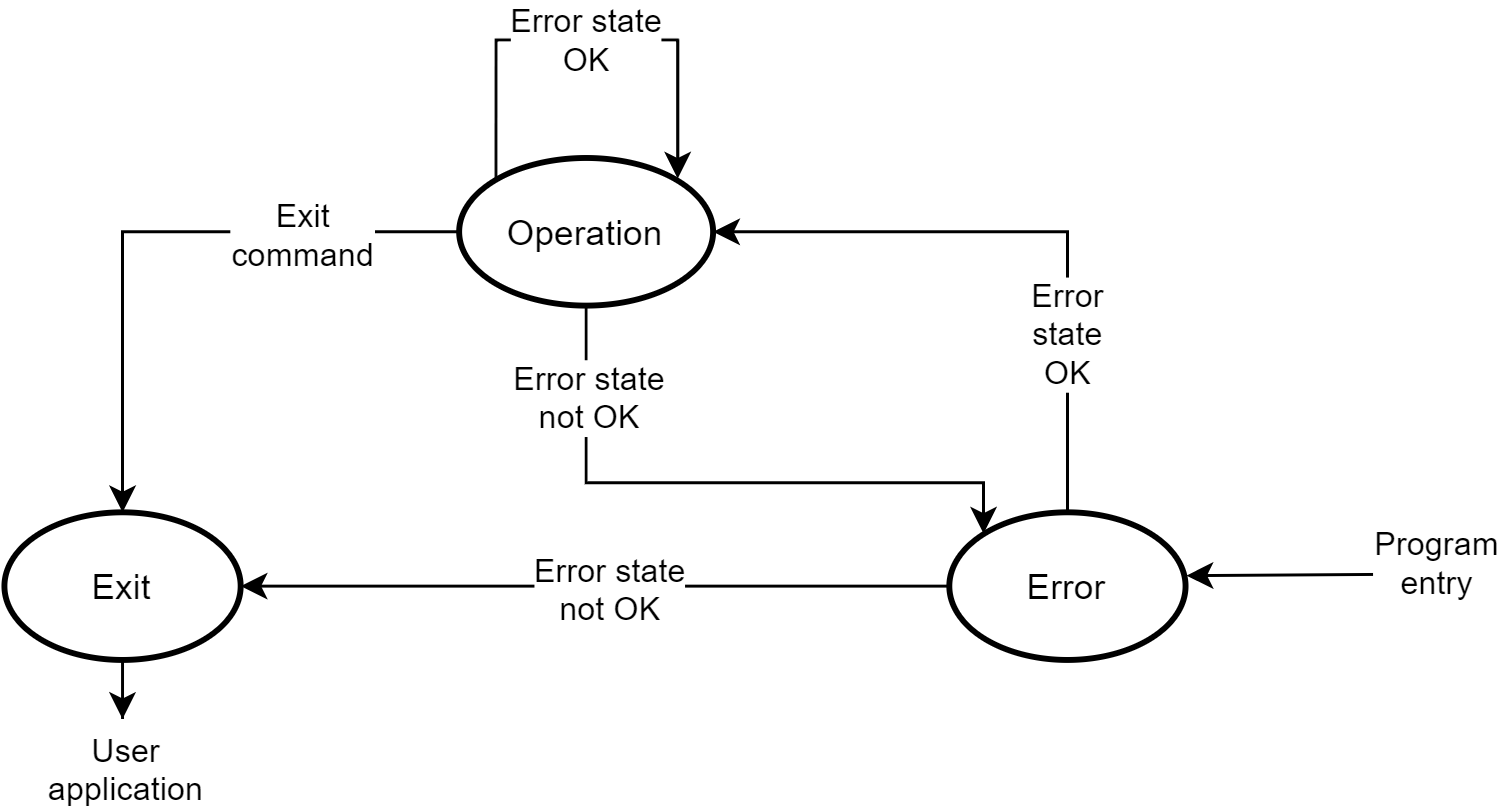
\includegraphics[width=.8\linewidth]{images/bootloader_flow.png}
    \captionof{figure}{State machine of the bootloader}
    \label{fig:bootloader_flow}
\end{figure}

\begin{figure}[H]
    \centering
    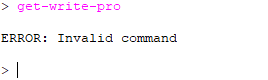
\includegraphics[width=.4\linewidth]{images/bootloader_cmd_err.png}
    \captionof{figure}{Example of an error from error state}
    \label{fig:bootloader_cmd_err}
\end{figure}

\section{Flash memory organization}

When using the bootloader the flash module is organized a shown in \autoref{tab:bootloader_flash}. 

\begin{table}[H]
\begin{tabular}{lllll}
\textbf{Block} & \textbf{Used by} & \textbf{Name} & \textbf{Block base addresses} & \textbf{Size} \\
 & \cellcolor[HTML]{D9D9D9} & \cellcolor[HTML]{D9D9D9}Sector   0 & \cellcolor[HTML]{D9D9D9}0x0800   0000 - 0x0800 3FFF & \cellcolor[HTML]{D9D9D9}16   Kbytes \\
 & \cellcolor[HTML]{D9D9D9} & \cellcolor[HTML]{D9D9D9}Sector   1 & \cellcolor[HTML]{D9D9D9}0x0800   4000 - 0x0800 7FFF & \cellcolor[HTML]{D9D9D9}16   Kbytes \\
 & \multirow{-3}{*}{\cellcolor[HTML]{D9D9D9}Bootloader} & \cellcolor[HTML]{D9D9D9}Sector   2 & \cellcolor[HTML]{D9D9D9}0x0800   8000 - 0x0800 BFFF & \cellcolor[HTML]{D9D9D9}16   Kbytes \\
 & Boot record & Sector   3 & 0x0800   C000 - 0x0800 FFFF & 16   Kbytes \\
 & \cellcolor[HTML]{D9D9D9} & \cellcolor[HTML]{D9D9D9}Sector   4 & \cellcolor[HTML]{D9D9D9}0x0801   0000 - 0x0801 FFFF & \cellcolor[HTML]{D9D9D9}64   Kbytes \\
 & \cellcolor[HTML]{D9D9D9} & \cellcolor[HTML]{D9D9D9}Sector   5 & \cellcolor[HTML]{D9D9D9}0x0802   0000 - 0x0803 FFFF & \cellcolor[HTML]{D9D9D9}128   Kbytes \\
 & \cellcolor[HTML]{D9D9D9} & \cellcolor[HTML]{D9D9D9}Sector   6 & \cellcolor[HTML]{D9D9D9}0x0804   0000 - 0x0805 FFFF & \cellcolor[HTML]{D9D9D9}128   Kbytes \\
 & \multirow{-4}{*}{\cellcolor[HTML]{D9D9D9}\begin{tabular}[c]{@{}l@{}}Current\\ application\end{tabular}} & \cellcolor[HTML]{D9D9D9}Sector   7 & \cellcolor[HTML]{D9D9D9}0x0806   0000 - 0x0807 FFFF & \cellcolor[HTML]{D9D9D9}128   Kbytes \\
 &  & Sector   8 & 0x0808   0000 - 0x0809 FFFF & 128   Kbytes \\
 &  & Sector   9 & 0x080A   0000 - 0x080B FFFF & 128   Kbytes \\
 &  & Sector   10 & 0x080C   0000 - 0x080D FFFF & 128   Kbytes \\
\multirow{-12}{*}{Main   memory} & \multirow{-4}{*}{\begin{tabular}[c]{@{}l@{}}New\\    \\ application\end{tabular}} & Sector   11 & 0x080E   0000 - 0x080F FFFF & 128   Kbytes \\
\rowcolor[HTML]{D9D9D9} 
\multicolumn{3}{l}{\cellcolor[HTML]{D9D9D9}System memory} & 0x1FFF   0000 - 0x1FFF 77FF & 30   Kbytes \\
\rowcolor[HTML]{D9D9D9} 
\multicolumn{3}{l}{\cellcolor[HTML]{D9D9D9}OTP area} & 0x1FFF   7800 - 0x1FFF 7A0F & 528   bytes \\
\rowcolor[HTML]{D9D9D9} 
\multicolumn{3}{l}{\cellcolor[HTML]{D9D9D9}Option bytes} & 0x1FFF   C000 - 0x1FFF C00F & 16   bytes
\end{tabular}
\caption{STM32F407 flash memory organization}
\label{tab:bootloader_flash}
\end{table}


\section{Application boot record}
\label{boot_record}

Aplication boot record is used to store meta data about the current user's application and new user's application. Meta data consists of: 
\begin{itemize}
    \item Checksum used for transmission,
    \item Application type used while transmitting,
    \item Length of application during transmission.
\end{itemize}
Boot record is also used to signalize that update of the application is needed to the bootloader. Flag is set when new application is successfully transmitted.

\autoref{memory_areas} and \autoref{app_boot_rec} show modifications added to the linker file needed to add the boot record. Address 0x800C000 is the starting address of sector 3 of the flash memory.

\begin{lstlisting}[frame=single, label={memory_areas}, caption={Memory areas from the linker file.}, captionpos=b]
/* Specify the memory areas */
MEMORY
{
RAM (xrw)      : ORIGIN = 0x20000000, LENGTH = 128K
CCMRAM (rw)      : ORIGIN = 0x10000000, LENGTH = 64K
/* Allow bootloader only first 3 sectors */
FLASH (rx)      : ORIGIN = 0x8000000, LENGTH = 48K 
/* Allow sector 3 for app boot record */
SEC3 (rx)		: ORIGIN = 0x800C000, LENGTH = 16K
}
\end{lstlisting}

\begin{lstlisting}[frame=single, label={app_boot_rec}, caption={Application boot record from the linker file.}, captionpos=b]
  /* Application boot record */
  .appbr 0x800C000 (NOLOAD):
  {
    . = ALIGN(4);
    _sappbr = .;       
    *(.appbr)
    *(.appbr*)
    
    . = ALIGN(4);
    _eappbr = .;   
  } >SEC3
\end{lstlisting}


\section{User application modifications}

On the start of every STM32F407 program is a vector table. Vector table contains numerous interrupt and exception vectors. List of all vectors is avaliable in \citep[p.~372]{stm32f407_ref_man}. On start up the program calls the vector on the address 4, the name of that vector is fittingly Reset handler. But before calling the reset handler main stack pointer(MSP) is set from the address 0. 

Because the program expects the main stack pointer and reset handler vector to be on the start of the program vector offset register(VTOR) is available. Vector offset register is simply added onto the flash memory base address to allow multiple programs in the same flash memory. Perfect for writing a bootloader!

To sum up, before bootloader jumps to the user application it must set the MSP to the one of the user's application then it jumps to the application's reset handler. Vector offset register can be set be the bootloader or in the user's application, former is chosen in this project.


\section{Command reference}

Important notices:

\begin{itemize}
 \item Every execute of a command must end with \textbackslash r \textbackslash n

 \item Commands are case insensitive
 
 \item On error bootloader returns "ERROR:<Explanation of error>"
 
 \item Optional parameters are surrounded with [] e.g. [example]

\end{itemize}

\noindent List of all commands:

\begin{itemize}

    \item \nameref{bl_cmd:version}
    \item \nameref{bl_cmd:help}
    \item \nameref{bl_cmd:reset}
    \item \nameref{bl_cmd:cid}
    \item \nameref{bl_cmd:get-rdp-level}
    \item \nameref{bl_cmd:jump-to}
    \item \nameref{bl_cmd:flash-erase}
    \item \nameref{bl_cmd:flash-write}
    \item \nameref{bl_cmd:mem-read}
    \item \nameref{bl_cmd:update-act} 
    \item \nameref{bl_cmd:update-new}
    \item \nameref{bl_cmd:en-write-prot}
    \item \nameref{bl_cmd:dis-write-prot}
    \item \nameref{bl_cmd:get-write-prot}
    \item \nameref{bl_cmd:exit}

\end{itemize}



\subsection{version - Gets a version of the bootloader.}
\label{bl_cmd:version}

Parameters:
\begin{lstlisting}
 - None
Execute command: 

    > version  
    
Response: 

    v1.0  
\end{lstlisting}
    
    
\subsection{help - Makes life easier.}
\label{bl_cmd:help}

\begin{lstlisting}
Parameters:

 -  None

Execute command: 

    > help  
    
Response: 

    <List of all available commands and examples>
\end{lstlisting}

\subsection{reset - Resets the microcontroller.}
\label{bl_cmd:reset}

\begin{lstlisting}
Parameters:

 - None

Execute command: 

    > reset
    
Response: 

    OK
\end{lstlisting}


\subsection{cid - Gets chip identification number.}
\label{bl_cmd:cid}

\begin{lstlisting}
Parameters:

 - None

Execute command: 

    > cid  
    
Response: 

    0x413
\end{lstlisting}

\subsection{get-rdp-level - Gets read protection \texorpdfstring{\protect\cite[p.~93]{stm32f407_ref_man}}{}}
\label{bl_cmd:get-rdp-level}

\begin{lstlisting}
Parameters:

  - None

Execute command: 

    > get-rdp-level  
    
Response: 

    level 0
\end{lstlisting}
    
\subsection{jump-to - Jumps to a requested address.}
\label{bl_cmd:jump-to}

\begin{lstlisting}
Parameters:

- addr - Address to jump to in hex format (e.g. 0x12345678), 0x can be omitted

Execute command: 

    > jump-to addr=0x87654321 
     
Response: 

    OK
\end{lstlisting}
     
\subsection{flash-erase - Erases flash memory.}
\label{bl_cmd:flash-erase}

\begin{lstlisting}
Parameters:

- type - Defines type of flash erase. "mass" erases all sectors, "sector" erases only selected sectors
    
- sector - First sector to erase. Bootloader is on sectors 0, 1 and 2. Not needed with mass erase
    
- count - Number of sectors to erase. Not needed with mass erase

Execute command: 

    > flash-erase sector=3 type=sector count=4 
     
Response: 

    OK
\end{lstlisting}

\subsection{flash-write - Writes to flash memory.}
\label{bl_cmd:flash-write}

\begin{lstlisting}
Parameters:

 - start - Starting address in hex format (e.g. 0x12345678), 0x can be omitted
     
 - count - Number of bytes to write, without checksum. Chunk size: 5120
 
 - [cksum] - Defines the checksum to use. If not present no checksum is assumed. WARNING: Even if checksum is wrong data will be written into flash memory!
 
      - "sha256" - Gives best protection (32 bytes), slowest, uses software implementation
           
      - "crc32" - Medium protection (4 bytes), fast, uses hardware implementation. Settings in [Apendix A](#apend_a)

      - "no" - No protection, fastest

Note:

  When using crc-32 checksum sent data has to be divisible by 4

Execute command: 

    > flash-write start=0x87654321 count=64 cksum=crc32  
    
Response: 

    chunks:1

    chunk:0|length:64|address:0x87654321

    ready
    
Send bytes:

    <64 bytes>
    
Response:

    chunk OK

    checksum|length:4

    ready
 
Send checksum:
     
     <4 bytes>
     
Response:
 
    OK
\end{lstlisting}

\subsection{mem-read - Read bytes from memory.}
\label{bl_cmd:mem-read}

\begin{lstlisting}
Parameters:

- start - Starting address in hex format (e.g. 0x12345678), 0x can be omitted
     
- count - Number of bytes to read

Execute command: 

    > mem-read start=0x87654321 count=3  
    
Response: 

    <3 bytes starting from the address 0x87654321>
    
Note:
- Entering invalid read address crashes the program and reboot is required. 
\end{lstlisting}

\subsection{update-act - Updates active application from new application memory area.}
\label{bl_cmd:update-act}

\begin{lstlisting}
Parameters:
- [force] - Forces update even if not needed

   - "true" - Force the update
                
   - "false" - Don't force the update


Execute command: 

    > update-act force=true
    
Response: 

    No update needed for user application
    Updating user application
    OK
\end{lstlisting}
    

\subsection{update-new - Updates new application.}
\label{bl_cmd:update-new}

\begin{lstlisting}
Parameters:

 - count - Number of bytes to write, without checksum. Chunk size: 5120
 
 - type - Type of application coding
       
      - "bin" - Binary format (.bin)
                
      - "hex" - Intel hex format (.hex)
      
      - "srec" - Motorola S-record format (.srec)
 
 - [cksum] - Defines the checksum to use. If not present no checksum is assumed. WARNING: Even if checksum is wrong data will be written into flash memory!
 
      - "sha256" - Gives best protection (32 bytes), slowest, uses software implementation
           
      - "crc32" - Medium protection (4 bytes), fast, uses hardware implementation. Settings in [Apendix A](#apend_a)

      - "no" - No protection, fastest


Execute command: 

    > update-new count=4 type=bin cksum=sha256
    
Response: 

    chunks:1

    chunk:0|length:4|address:0x08080000

    ready
    
Send bytes:

    <4 bytes>
    
Response:

    chunk OK

    checksum|length:32

    ready
 
Send checksum:
     
     <32 bytes>
     
Response:
 
    OK
\end{lstlisting}

\subsection{en-write-prot - Enables write protection per sector.}
\label{bl_cmd:en-write-prot}

\begin{lstlisting}
Parameters:

- mask - Mask in hex form for sectors where LSB corresponds to sector 0

Execute command: 

    > en-write-prot mask=0xFF0
    
Response: 

    OK
\end{lstlisting}
    
\subsection{dis-write-prot - Disables write protection per sector.}
\label{bl_cmd:dis-write-prot}

\begin{lstlisting}
Parameters:

- mask - Mask in hex form for sectors where LSB corresponds to sector 0

Execute command: 

    > dis-write-prot mask=0xFF0
    
Response: 

    OK
\end{lstlisting}

\subsection{get-write-prot - Returns bit array of sector write protection.}
\label{bl_cmd:get-write-prot}Parameters:

\begin{lstlisting}
- None

Execute command: 

    > get-write-prot
    
Response: 

    0b100000000010
\end{lstlisting}

\subsection{exit - Exits the bootloader and starts the user application.}
\label{bl_cmd:exit}

\begin{lstlisting}
Parameters:

- None

Execute command: 

    > exit  
    
Response: 

    Exiting
\end{lstlisting}
